\documentclass{article}
\usepackage[a4paper, total={6in, 8in}]{geometry}
\usepackage{amsmath,amsthm,amssymb}
\usepackage[shortlabels]{enumitem}
\usepackage[utf8]{inputenc}
\usepackage{sectsty}
\usepackage{listings}
\usepackage{xcolor}
\lstset { %
    language=C++,
    backgroundcolor=\color{black!5}, % set backgroundcolor
    basicstyle=\footnotesize,% basic font setting
}

\usepackage{mathtools}
\DeclarePairedDelimiter\ceil{\lceil}{\rceil}
\DeclarePairedDelimiter\floor{\lfloor}{\rfloor}

\theoremstyle{definition}
\newtheorem{problem}{Problem}[section]
\newtheorem{exercise}{Exercise}[section]

\sectionfont{\fontsize{12}{15}\selectfont}

\title{Problem Set 1}
\author{Jose Chavez}
\begin{document}
\maketitle


\section{Ordering functions}

\begin{exercise}
    Arrange the following functions in increasing order of growth rate and justify your answer through a proof. 

    \begin{enumerate}[a)]
        \item $2^n$
        \item $\log_2 n$
        \item $n^{\log_2n}$
        \item $2^{n^2}$
        \item $2^{2^n}$
    \end{enumerate} 

    The order is as follow:
    \begin{center}
        $\log_2n<n^{\log_2n}<2^n<2^{n^2}<2^{2^n}$
    \end{center}
    \begin{enumerate}
        \item \textit{Proof} of $\log_2n<n^{\log_2n}$\\
            We say $a=\log_2n$ , then
            \begin{center}
                $an < n^a$ ; for every $a\geqslant0$
            \end{center}
        \item \textit{Proof} of $2^n<2^{n^2}$\\
            As the bases are the same we just compare the exponents
            \begin{center}
                $n<n^2$
            \end{center}
        \item \textit{Proof} of $2^{n^2}<2^{2^n}$\\
            As the bases are the same we just compare the exponents
            \begin{center}
                $n^2<2^n$
            \end{center}
            We know that it holds when $n\geqslant5$\\
            So we will Assume is true an we will try to proof it with $n+1$
            \begin{align*}
                n^2&<2^{n+1}\\
                &<2^n*2
            \end{align*}
            We can multiply by 2 our first term, so it will because
            \begin{center}
                $(n+1)^2<2 * n^2 < 2 * 2^n$
            \end{center}
            we know that $(n-1)^2 \geqslant 4^2 > 2$ since $n\geqslant5$ so we will expand that inequality
            \begin{align*}
                (n-1)^2 &> 2\\
                n^2 - 2n -1 &>0\\
                2n^2 -2n -1 &>n^2\\
                2n^2 &> n^2 + 2n +1\\
                2n^2 &> (n+1)^2\\
            \end{align*}

        
        
        
    \end{enumerate}
\end{exercise}

\section{$O$, $\Theta$ and $\Omega$ exercises that were definitely not taken from CLRS}


\begin{exercise}
    % taken from cormen, symmetric property

    Prove or disprove: $f(n) = \Theta(g(n))$ if and only if $g(n) = \Theta(f(n))$.

    Assuming the first statement is true. And by $\Theta$ definition we have

    \begin{align*}
    c_1g(n)\leqslant &f(n) \leqslant c_2g(n)\\
    g(n) &\leqslant 1/c_1f(n)\\
    1/c_2f(n) &\leqslant g(n)
    \end{align*}    

    Taking a $z_1 = 1/c_1$ y $z_2=1/c_2$ we have
    \begin{align*}
        z_2f(n) \leqslant g(n) \leqslant z_1g(n)\\
    \end{align*}
    
    we proof that $g(n) \in \Theta(f(n))$
        
\end{exercise}

\begin{exercise}
    % taken from cormen, symmetric property

    Prove or disprove: $f(n) = \Theta(f(n))$.

    We start by assuming that $f(n) = \Theta(f(n))$ is true. So 
    $c_1f(n) \leqslant f(n) \leqslant c_2f(n)$.
    Then we must proof that $f(n)= \Omega(n)$ and $f(n)= O(n)$. We use such definitions\\    
    \begin{center}
    $0 \leqslant c_1f(n) \leqslant f(n)$ and 
    $f(n)\leqslant c_2f(n)$
    \end{center}
    Thus,\\
    \begin{align*}
        c_1f(n) &\leqslant c_2f(n)\\
        c_1 &\leqslant c_2
    \end{align*}

    From our definiton $f(n)= \Omega(n)$ and $f(n)= O(n)$ holds when $c_1 \leqslant c_2$ .
    Thus , $f(n) = \Theta(f(n))$.

    
\end{exercise}

\begin{exercise}
    % taken from cormen
    Using the basic definition of $\Theta$-notation, prove that $\max(f(n), g(n)) = \Theta(f(n) + g(n))$.\\
    We will see two ways of proving it.

    First using the definition we can say
    \begin{center}
        $c_1(f(n)+g(n)) \leqslant max(f(n),g(n)) \leqslant c_2(f(n)+g(n))$        
    \end{center}
    \begin{align*}
        max(f(n),g(n)) &\leqslant 1(f(n)+g(n))\\
        max(f(n),g(n)) &\geqslant 1/2(f(n)+g(n))\\
    \end{align*}
    So it holds true for $c_1 \leqslant 1/2 $ and $c_2 \geqslant 1$ .\\

    The other approach will be:\\
    Note that $f(n)\leqslant f(n)+g(n)$ and $g(n)\leqslant f(n)+g(n)$ . Hence
    \begin{center}
        $max(f(n),g(n)) = O(f(n)+g(n))$
    \end{center}
    Now note that if $f(n) \geqslant g(n)$ , we can say $f(n)+f(n)\geqslant f(n)+g(n)$ , this equals  $2(f(n)) \geqslant f(n)+g(n)$. We will use the same strategie if $g(n) \geqslant f(n)$.
    Hence we have
    \begin{center}
        $f(n)+g(n) \leqslant 2 max(f(n),g(n))$
    \end{center}
    Therefor
    \begin{center}
        $max(f(n),g(n)) = \Omega(f(n)+g(n))$ 
    \end{center}
    Thus
    \begin{center}
        $max(f(n),g(n)) = \Theta(f(n)+g(n))$ 
    \end{center}
\end{exercise}

\begin{exercise}
    % Taken form Knuth Concrete Mathematics S9.6 EX5

    Prove or disprove: $O(f(n) + g(n)) = f(n) + O(g(n))$, if $f(n)$ and $g(n)$.
\end{exercise}

% next three are taken from tardos properties of asymptotic growth rates
\begin{exercise}
    Prove or disprove: If $f(n) = O(g(n))$ and $g(n) = O(h(n))$, then $f(n) = O(h(n))$.

    Based on the definitions we have
    \begin{center}
        $f(n)\leqslant c_1g(n)$ and $g(n)\leqslant c_2h(n)$\\
        $f(n)\leqslant c_xh(n)$        
    \end{center}
    We arrange the inequalities then we multiply by $c_1$ the following expressions without interfering with the inequality
    \begin{align*}
        f(n) \leqslant g(n) &\leqslant c_1g(n) \leqslant c_2h(n)\\
        c_1g(n) &\leqslant c_1c_2h(n)\\
        f(n) &\leqslant c_1c_2h(n)\\
    \end{align*}
    Then by reverse-defintion we have
    \begin{center}
        $f(n)=O(h(n))$\\
        $f(n) \leqslant c_xh(n)$
    \end{center}
    that holds true when  $c_x \geqslant c_1c_2$
\end{exercise}

\begin{exercise}
    Prove or disprove: Suppose that $f(n)$ and $g(n)$ are two functions such that for some other function $h(n)$, we have $f(n) = O(h(n))$ and $g(n) = O(h(n))$. Then $f(n) + g(n) = O(h(n))$.
    Based on the definitions we have
    \begin{center}
        $f(n)\leqslant c_1h(n)$ and $g(n)\leqslant c_2h(n)$\\
        $f(n)+g(n) \leqslant (c_1+c_2)h(n)$
    \end{center}
    And by using $O$ defintion, we have
    \begin{align*}
        f(n)+g(n) &= O(h(n))\\
        f(n)+g(n) &\leqslant c_3h(n)\\
    \end{align*}
    It holds as long as $c_3=c_1+c_2$
\end{exercise}

\begin{exercise}
    Prove or disprove: Let $k$ be a fixed constant, and let $f_1(n), f_2(n), \ldots, f_k(n)$ and $h(n)$ be functions such that $f_i(n) = O(h(n))$ for all $i$. Then $f_1(n) + f_2(n) + \cdots + f_k(n) = O(h(n))$.
\end{exercise}

\section{Solving Recurrences}

\begin{exercise}
    Use the Master Theorem to give an asymptotic upper bound for $T(n)$ in each of the following recurrences. Assume that $T(n)$ is constant for $n \leq 2$. Make your bounds as tight as possible.
    \begin{enumerate}[a)]
        \item $T(n) = 4T(n/4) + 5n \Longrightarrow T(n)=O(n\log n)$
        \item $T(n) = 4T(n/5) + 5n \Longrightarrow T(n)=O(n)$
        \item $T(n) = 5T(n/4) + 4n \Longrightarrow T(n)=O(n^{\log_4 5})$
        \item $T(n) = 25T(n/5) + n^2 \Longrightarrow T(n)=O(n^2\log n)$
        \item $T(n) = 4T(\sqrt{n}) + \log^5n \Longrightarrow T(n)=O(\log^5 n)$
        \item $T(n) = T(\sqrt{n}) + 5 \Longrightarrow T(n)=O(\log\log n)$
    \end{enumerate}
\end{exercise}

\begin{exercise}
    Use the Recurrence Tree (optional, but really helpful sometimes) to guess an upper bound and prove it using the Substitution Method. 
    \begin{enumerate}[a)]
        \item $T(n) = 2T(n-1) + 1$\\
            Guess: $O(2^n)$\\
            I.H: $T(n) \leqslant \textit{c}2^n-d$\\
            I.S: 
            \begin{align*}
                T(n-1) &\leqslant 2(c 2^{n-1}-d)+1\\
                &=  c2^n-2d+1\\
                &\leqslant c2^n -d \quad\text{;  when $d > 0$}               
            \end{align*}
            
        \item $T(n) = 2T(n-1) - 1$\\
        Guess: $O(2^n)$\\
        I.H: $T(n) \leqslant \textit{c}2^n$\\
        I.S: 
        \begin{align*}
            T(n-1) &\leqslant 2(c 2^{n-1})-1\\
            &=  c2^n-1\\
            &\leqslant c2^n                 
        \end{align*}
        \item $T(n) = T(n/2) + T(n/4) + n^2$\\
        Guess: $O(n^2)$\\
        As we are trying to prove an upper bound we can stablish that our second term is $T(n/2)$ because $T(n/2)>T(n/4)$ so we can fix our recurrence 
        \begin{center}
            $T(n)=2T(n/2)+n^2$
        \end{center}
        I.H: $T(n) \leqslant \textit{c}n^2$\\
        I.S: 
        \begin{align*}
            T(n/2) &\leqslant 2(c(n/2)^2)+n^2\\
            &=  cn^2/2 + n^2\\
            &=  (2n^2+cn^2)/2\\
            &= ((2+c)/2)n^2\\
            &\leqslant c2^n  \quad\text{;  when $c\geqslant2$}               
        \end{align*}
        \item $T(n) = 2T(\floor*{n/2} + 16) + n$
    \end{enumerate}
\end{exercise}

\section{\textit{Spooky Problems}}

\begin{problem}

    Our friend Martin is moving to Barranco. He is a big fan of beer and pretty much anything that contains alcohol. Luckily, he has found a street with $n$ bars. Since he will definitely visit all of them frequently, he wants to find an apartment close to them. 

\bigbreak\noindent Martin wants to minimize the total distance to all of the bars and has offered you a \textit{ronnie} to come up with an algorithm to solve his problem.

\bigbreak\noindent Let $n$ be the number of bars in the street and the let the following sequence represent the street numbers where they are: $s_1, s_2, \ldots, s_i, \ldots, s_n$. Note that several bars might be in the same location/street number.
    
\bigbreak\noindent Both $n$ and the sequence of $s_i$'s are integers. The distance between two street numbers $s_i$ and $s_j$ is $d_{ij} = |s_i - s_j|$.

    \begin{enumerate}[a)]
        \item Find an $O(n\log n)$ solution.
        \item \textit{Bonus}: Can you do better? Sketch a faster algorithm.
    \end{enumerate}
\end{problem}

\begin{problem} 
    Solve \texttt{UVa 10077: The Stern-Brocot Number System}.\\
    \begin{figure}[!ht]
        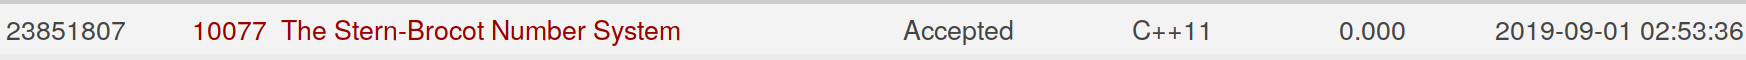
\includegraphics[width=\textwidth]{10077.png}
    \end{figure} 
    \begin{lstlisting}
#include <iostream>
#include <vector>

class Node
{
public:
    double up, down;

    Node() = default;
    bool operator==(Node const &node)
    {
        if (node.up == up && node.down == down)
            return true;
        return false;
    }
    bool operator<(Node const &node)
    {
        if (node.up / node.down > up / down)
            return true;
        return false;
    }
    bool operator>(Node const &node)
    {
        if (node.up / node.down < up / down)
            return true;
        return false;
    }
    Node operator+(Node const &node)
    {
        Node newNode{node.up + up, node.down + down};
        return newNode;
    }
};

std::string find(Node node)
{
    Node left{0, 1};
    Node middle{1, 1};
    Node right{1, 0};

    std::string path;

    while (true)
    {
        if (node == middle)
            return path;
        if (node < middle)
        {
            Node temp = middle;
            right = middle;
            middle = temp + left;
            path += 'L';
        }
        if (node > middle)
        {
            Node temp = middle;
            left = middle;
            middle = temp + right;
            path += 'R';
        }
    }
}

int main()

{

    double div1, div2;
    std::cin >> div1 >> div2;
    while (true)
    {
        if (div1 == 1 and div2 == 1)
            break;
        Node a1{div1, div2};
        std::cout << find(a1) << '\n';
        std::cin >> div1 >> div2;
    }
    return 0;
}
    \end{lstlisting}
\end{problem}

\end{document}